% ============================================================
%  Post-disaster population recovery — Nature Communications format
%  Working draft v0.2
% ============================================================
\documentclass[11pt]{article}

% ---- packages ----
\usepackage[utf8]{inputenc}
\usepackage[T1]{fontenc}
\usepackage{mathptmx}
\usepackage[margin=2.5cm]{geometry}
\usepackage{amsmath,amssymb}
\usepackage{graphicx}
\usepackage{booktabs}
\usepackage{natbib}
\usepackage{xcolor}
\usepackage{hyperref}
\usepackage[font=small,labelfont=bf]{caption}
\usepackage{enumitem}
\setlist{nosep,leftmargin=*}
\usepackage{placeins}   % \FloatBarrier to keep floats inside sections

% ---- shortcuts ----
\newcommand{\dnear}{\delta_{\mathrm{near}}}
\newcommand{\dpeak}{D_{\mathrm{peak}}}
\newcommand{\apred}{\alpha_{\mathrm{pred}}}
\newcommand{\aemp}{\alpha_{\mathrm{emp}}}
\newcommand{\Ds}{D_s}
\newcommand{\Dnorm}{D_{\mathrm{norm}}}
\newcommand{\rhosp}{\rho}             % Spearman rho
\newcommand{\Dpred}{D_{\mathrm{pred}}}
\newcommand{\Demp}{D_{\mathrm{emp}}}

% ---- placeholder figure command ----
\newcommand{\placeholderfig}[2]{%
  \begin{center}
    \fcolorbox{black!30}{black!5}{\parbox{0.9\linewidth}{\centering\vspace{1.2cm}%
    \textbf{Figure~#1}\\\smallskip\small #2 \vspace{1.2cm}}}
  \end{center}
}

% ============================================================
\title{\textbf{Displacement geometry and amplitude\\
predict post-disaster population recovery}}

\author{
  Jin Lin$^{1,\ast}$
  \and Second Author$^{1}$
  \and Third Author$^{2}$
  \\[6pt]
  {\small $^{1}$Affiliation One}\\
  {\small $^{2}$Affiliation Two}\\
  {\small $^{\ast}$Corresponding author.\ E-mail: xxx@xxx.edu}
}
\date{}

% ============================================================
\begin{document}
\maketitle
\thispagestyle{empty}

% ============================================================
%  ABSTRACT
% ============================================================
\begin{abstract}
\noindent
  Natural disasters displace millions annually, yet what determines how
  quickly populations recover remains poorly understood. Here we analyze
  displacement across 16 disasters -- earthquakes, hurricanes, floods,
  and wildfires in 11 countries -- using Facebook Disaster Maps.
  Recovery rates vary by more than an order of magnitude.  We show that
  this variation is predicted by two independent quantities, both
  measurable at peak displacement.  The spatial geometry of the
  displacement profile---whether populations scatter outward or
  concentrate near the epicenter---predicts recovery rate
  ($\rho = -0.53$, $p = 0.036$).  A diffusion--relaxation model
  explains the link: spatial diffusion selectively damps finer-scale
  components, so evacuation-type perturbations with steep gradients
  relax faster.  Independently, perturbation amplitude predicts recovery:
  larger disruptions recover faster ($\rho = +0.60$, $p = 0.014$), a
  counterintuitive scaling invariant to national-level development
  indicators.  Together, geometry and amplitude encode the recovery
  trajectory in the initial condition, reframing post-disaster recovery
  as governed by the physics of population redistribution.
\end{abstract}

\bigskip

% ============================================================
%  INTRODUCTION
% ============================================================
\section*{Introduction}

Natural disasters triggered over 45~million internal displacements in
2024 alone~\citep{IDMC2025}, and the proportion of the global
population exposed to floods alone has grown substantially over the
past two decades~\citep{Tellman2021}, a figure that has risen sharply
over recent decades.  How quickly displaced populations recover determines
the duration of humanitarian need, the trajectory of reconstruction,
and the long-term social fabric of affected
communities~\citep{Aldrich2012,Cutter2003}.  Yet despite a rapidly
growing body of quantitative research~\citep{Lu2012,Yabe2020,Huang2025},
no general framework exists to predict whether a displaced population
will return within days or remain uprooted for months.

Quantitative tracking of post-disaster displacement---building on the
scaling laws that characterize routine human
mobility~\citep{Brockmann2006,Song2010}---has advanced rapidly with
mobile phone and social-media data.  Call detail records enabled
near-real-time monitoring
after the 2010 Haiti earthquake~\citep{Lu2012,Bengtsson2011} and the
2015 Nepal earthquake~\citep{Wilson2016}; survey data revealed the
complexity of disaster-induced migration in
Bangladesh~\citep{GrayMueller2012}; network approaches showed that
pre-disaster social connectivity shapes recovery
trajectories~\citep{Yabe2020}; and high-resolution social-media data
enabled quantification of displacement and migration dynamics
across entire island populations after Hurricane
Maria~\citep{Acosta2020}.  These studies document a recurring pattern: an acute displacement
followed by gradual return, with rates that appear to vary widely across
events and countries~\citep{Huang2025}.  Recent work has begun to
characterise systematic recovery patterns---identifying rapid,
slow, and non-recovering trajectories across flood events in
China~\citep{Tang2023} and classifying recovery archetypes across
multiple disaster types in Japan~\citep{Yabe2020b}---while CDR-based
analyses of the 2023 T\"{u}rkiye--Syria earthquake have revealed
heterogeneous displacement patterns at the sub-regional
scale~\citep{Aydogdu2025}.  The studies are, however, largely confined
to single events or single hazard types, making it difficult to
determine whether observed recovery differences reflect systematic
physical properties of the disturbance or merely idiosyncratic
event-specific contingencies.  The dominant resilience
framework attributes recovery speed to the latter---coping capacity,
institutional quality, infrastructure
stock~\citep{Cutter2003,Aldrich2012}---predicting that wealthier,
better-governed societies should recover systematically faster.

Post-disaster displacement is, at its core, a spatial perturbation of a
population field followed by relaxation toward equilibrium.  Human
mobility flows can be described as gradient-driven processes in a
continuous spatial field~\citep{Mazzoli2019,GomezGardenes2018,Lenormand2015}:
when the field is perturbed, restoring fluxes emerge that depend on
the spatial structure of the perturbation.  Statistical-physics models
show that both individual trajectories and aggregate population flows
obey universal scaling laws that emerge from a small set of
mechanisms~\citep{Yan2017}.  In such diffusive systems, the
relaxation rate is set by the spatial frequency content of the initial
condition---finer-scale disturbances decay at progressively faster
rates~\citep{Crank1975}.  Empirically, crisis-induced mobility
deviations exhibit stable decay dynamics consistent with relaxation
toward equilibrium, across event types and spatial
scales~\citep{Li2022}.  Displacement therefore has not
only an \emph{amplitude}---how severely the population is disturbed---but
a \emph{geometry}: the spatial pattern of where people are displaced to
and from.  If the physical analogy holds, recovery speed should depend on
the spatial geometry of the displacement profile at peak time.

Using Facebook Disaster Maps~\citep{Maas2019,Jia2020}, which provide
standardized 8-hour population displacement estimates across all
activated events worldwide, we construct an aggregated displacement
metric~$D(t)$ for 16~events spanning four hazard types in 11~countries
(Materials and Methods).  The dataset covers events ranging from the
2023 T\"{u}rkiye--Syria earthquake, which displaced millions within
hours, to smaller wildfires in the western United States---a 50-fold
range in peak displacement amplitude and an order-of-magnitude spread
in recovery speed.  We find that recovery speed is jointly predicted by
two physically distinct and statistically independent quantities, both
measurable at peak displacement.  The spatial geometry of the
displacement profile---summarized by the near-field displacement
direction~$\dnear$---determines recovery rate: events that scatter
population outward recover faster, a signal reproduced by a minimal
diffusion--relaxation PDE acting through mode-selective damping.
Independently, the perturbation amplitude~$\dpeak$ shows a
counterintuitive positive association with recovery speed---larger
disruptions recover faster---and this scaling is invariant to national
HDI, GDP per capita, and INFORM Risk scores.  Together, these findings
reframe
post-disaster recovery as a process governed by the physics of
population redistribution: the spatial pattern of where people go at
peak time encodes how quickly they come back.


% ============================================================
%  RESULTS
% ============================================================
\section*{Results}

% ---- R1 ----
\subsection*{Universal relaxation at diverse recovery rates}

Across all 16~events (Supplementary Table~S1), the aggregated
displacement metric~$D(t)$ traces the same qualitative arc: a rapid rise
to a peak followed by gradual decay (Fig.~\ref{fig:relaxation}b).  This
pattern is universal despite dramatic heterogeneity in the underlying
physical process: the 2023 T\"{u}rkiye--Syria earthquake unleashed
ground rupture across 300~km of fault, displacing nearly half the
regional population within 24~hours; the 2024 Boise County wildfire in
Idaho evacuated communities progressively as the fire perimeter expanded
over several days; the 2020 Bangladesh monsoon flood displaced
households incrementally over days.  In each case, $D(t)$ collapses
event-specific mechanisms into a single scalar trajectory of
perturbation and relaxation, consistent with the aggregated
displacement arcs identified in CDR-based studies of other
seismic events~\citep{Giardini2023}.

Recovery speeds, however, diverge dramatically.  Normalized decay
curves fan out across events on log--log axes
(Fig.~\ref{fig:relaxation}c): the decay rate~$\alpha$ varies by more
than an order of magnitude, from near-zero (negligible recovery over two
weeks) to above unity (rapid return within days).  The T\"{u}rkiye--Syria
earthquake, for instance, shows one of the slowest recoveries in the
dataset, with population displacement persisting substantially through
the two-week observation window; the Boise County wildfire shows among
the fastest, with $D(t)$ returning to near-baseline within four to five
days.  Fast and slow recoveries occur within each hazard type
(Fig.~\ref{fig:relaxation}c): a Kruskal--Wallis test rejects no
difference among hazard groups ($H = 2.61$, $p = 0.63$;
Supplementary~\S6.6), confirming that within-group variation dominates
over between-group variation.

The decay rates are robust to measurement choices (Supplementary
Table~S2).  Events with faster decay also converge to genuinely lower
residual levels: $\rho(\aemp, D_\infty) = -0.703$, $p = 0.002$
(Fig.~\ref{fig:relaxation}d),
where~$D_\infty$ is the mean of normalised~$D(t)$ over the post-peak
tail (Supplementary \S6.4).  If~$\alpha$ merely captured an initial transient---a fast drop
followed by a high plateau---we would expect no relationship, or even
a positive correlation, between~$\alpha$ and~$D_\infty$.  The strong
anticorrelation indicates that fast-decaying events also converge to
lower residuals: populations that leave quickly also return more
completely.

\begin{figure}[t]
\centering
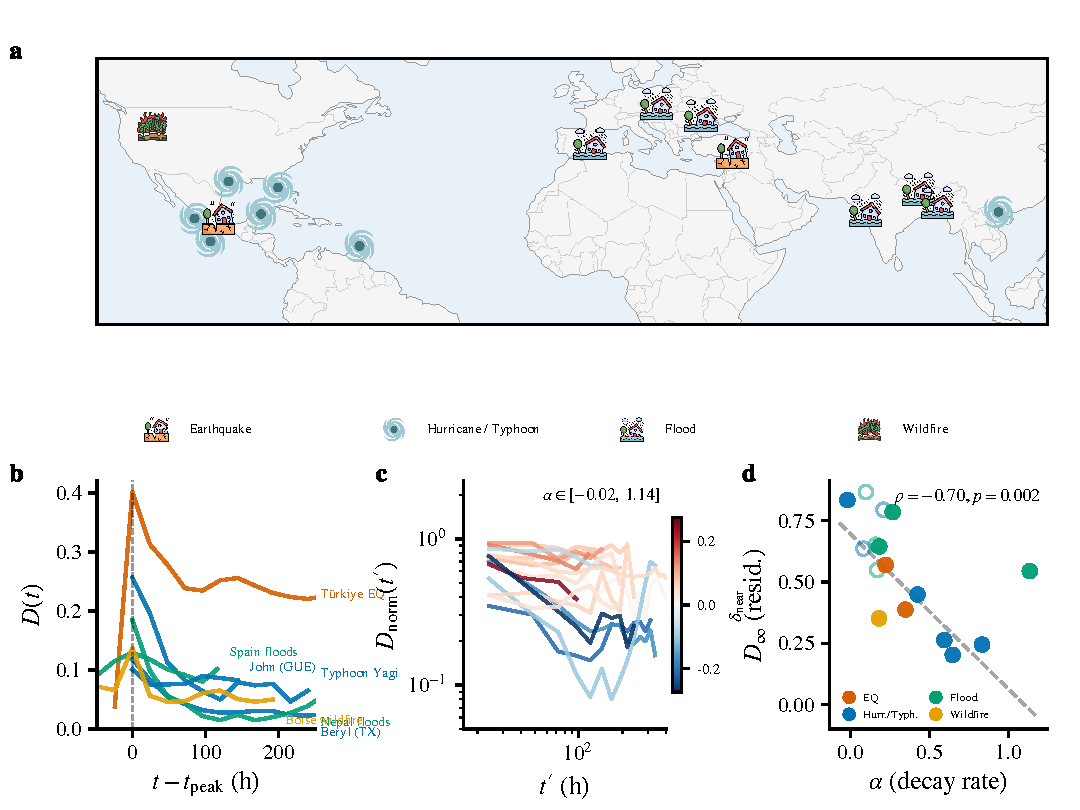
\includegraphics[width=\textwidth]{figures/fig1_universal_relaxation.pdf}
\caption{\textbf{Post-disaster displacement relaxes universally but at diverse rates.}
\textbf{(a)}~Global map of the 16~events spanning four hazard types and three
continents; icons indicate hazard type.
\textbf{(b)}~$D(t)$ time series for seven representative events (coloured by
hazard type), showing the sharp peak and subsequent power-law relaxation.
\textbf{(c)}~All 16~events normalised by peak displacement on log--log axes
and coloured by $\dnear$; the spread in slopes reveals an order-of-magnitude
range in $\alpha \in [-0.02,\;1.14]$.
\textbf{(d)}~$\alpha$ versus~$D_\infty$ (residual displacement fraction at
the end of the observation window); faster-decaying events also converge to
lower residual levels ($\rhosp = -0.70$, $p = 0.002$), validating $\alpha$
as a meaningful recovery indicator rather than a transient artifact.
Open markers: $R^2 < 0.75$.}
\label{fig:relaxation}
\end{figure}

% ---- R2 ----
\FloatBarrier
\subsection*{Displacement geometry predicts recovery speed}

To identify what drives the variation in~$\alpha$, we examine how population density is redistributed at peak displacement.  The radial profile
captures how population density is redistributed as a function of
distance from the epicenter. We summarise its near-field character by
a single scalar,~$\dnear$: the mean population-density deviation within
50~km (Materials and Methods). Negative values indicate net outward
evacuation (hereafter EVAC); positive values indicate net influx toward
the epicenter (hereafter INFL).

The contrast between these two displacement geometries is visible in the
representative radial profiles (Fig.~\ref{fig:shape}b).  Hurricane Beryl
in southeastern Texas---an evacuation-type event ($\dnear < 0$)---shows
a strongly negative near-field signature: population
is displaced outward, creating a sharp deficit within 50~km that approaches
near-zero deviation by about 100~km. By contrast, the 2024 Spain flood---an
influx-type event ($\dnear > 0$)---shows a positive near-field anomaly and
a smoother radial gradient through the mid-field. These two contrasting geometries---
steep evacuation versus smooth influx---correspond systematically to fast
and slow recovery, respectively.  Identification of spatial evacuation
patterns from mobility data has precedent in other
hurricane contexts~\citep{Li2024Evacuation}.

Events that scatter population outward at peak time recover faster
($\rhosp = -0.53$, $p = 0.036$; Fig.~\ref{fig:shape}a).  In plain
terms: when a disaster pushes people away from the epicenter---creating a
pronounced zone of population deficit in the near-field---the subsequent
return to baseline is rapid.  Conversely, when displaced populations
concentrate near the epicenter, recovery is slow.  The near-field
displacement direction~$\dnear$, a single number measurable at peak time,
separates fast from slow recoveries across all four hazard types.

The strongest signal comes not from the innermost ring but from the
mid-field (50--100~km): $\rhosp = -0.733$, $p = 0.025$ among the
$n = 9$ events with sufficient spatial coverage in that annulus
(Supplementary \S5).  This is consistent with an evacuation
shadow---the zone of suppressed population density that forms as
residents flee outward---being most pronounced at intermediate
distances.  We retain~$\dnear$ (0--50~km) as the primary predictor
because it maximises sample coverage ($n = 16$) while capturing the
same physical signal.

The association holds under multiple robustness tests: it persists
across four fixed time-window definitions
($[24,72]$~h through $[24,144]$~h), Theil--Sen estimation, a
model-free decay ratio~$D(72)/D(24)$, and sensitivity to the near-field
radius~$r_{\mathrm{near}}$ from 10 to 200~km (Supplementary Table~S2,
Supplementary \S6.3; Fig.~\ref{fig:shape}d).  Jackknife resampling
(leave-one-out, $n = 16$ iterations) yields a 95\% interval
of $[-0.62,\,-0.44]$ for the $\aemp$--$\dnear$ correlation
(Fig.~\ref{fig:shape}c), confirming that no single event drives the signal.

\begin{figure}[t]
\centering
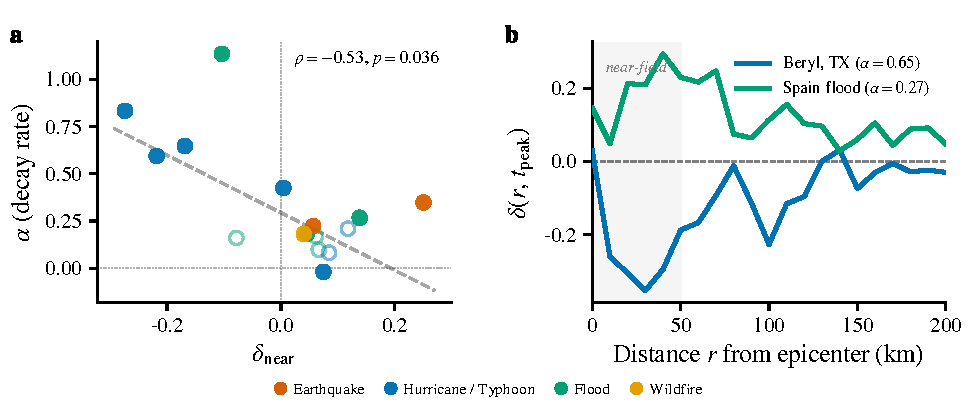
\includegraphics[width=\linewidth]{figures/fig2_shape_predicts_recovery.pdf}
\caption{\textbf{Displacement geometry predicts recovery speed.}
\textbf{(a)}~$\alpha$ versus $\dnear$ with Theil--Sen regression line;
open markers denote events with $R^2 < 0.75$.
\textbf{(b)}~Representative radial profiles at peak time for a fast-recovering
EVAC event (Hurricane Beryl in southeastern Texas, $\dnear < 0$) and a
slow-recovering INFL event (2024 Spain flood, $\dnear > 0$); shaded region
marks the near-field ($r < 50$~km).
\textbf{(c)}~Jackknife leave-one-out distribution of $\rhosp(\alpha, \dnear)$;
shaded band is the 95\% interval $[-0.62,\,-0.44]$.  The
vertical line marks the full-sample estimate $\rhosp = -0.53$; no single
event drives the correlation.
\textbf{(d)}~Parameter sensitivity: $p$-value (Mann-Whitney EVAC vs INFL $\alpha$)
under three robustness choices ($r_{\max}$, near-field threshold,
bounce tolerance).  All settings except the most stringent yield $p < 0.05$
(vertical dashed line), confirming the EVAC--INFL contrast as an
auxiliary check; primary inference uses the continuous
$\rhosp(\alpha,\dnear)$ association (Supplementary Table~S2).}
\label{fig:shape}
\end{figure}


% ---- R3: PDE mechanism ----
\FloatBarrier
\subsection*{A diffusion--relaxation model explains the shape--rate
connection}

Why should the spatial shape of displacement determine recovery speed?
We propose a minimal diffusion--relaxation equation for the radial
displacement field~$\delta(r,t)$:
\begin{equation}
  \frac{\partial\delta}{\partial t}
    = \frac{\Ds}{r}\frac{\partial}{\partial r}
      \!\left(r\,\frac{\partial\delta}{\partial r}\right)
    - k\,\delta,
  \label{eq:pde}
\end{equation}
where $\Ds$ is a spatial diffusion coefficient and $k$ a uniform
relaxation rate.  Under zero-flux boundary conditions, the solution
decomposes into radial Bessel modes $J_0(\mu_n r / R)$, each decaying
at rate $\lambda_n = k + \Ds(\mu_n/R)^2$ (Materials and Methods; Fig.~\ref{fig:pde}b).  Higher-order
modes---encoding finer spatial structure---decay at progressively
faster rates.

The physical intuition follows the modal decomposition
(Fig.~\ref{fig:pde}a,b).  An evacuation-type profile---population
removed from the near-field and redistributed outward---creates a steep
radial gradient at small~$r$, requiring substantial weight in
high-order Bessel components ($n \geq 2$).  Because mode-$n$ decay
scales as $\lambda_n \propto \mu_n^2$ and $\mu_n$ increases roughly
linearly with $n$, high-$n$-dominated initial conditions relax faster
than smooth profiles dominated by the lowest-order modes.  By
contrast, an influx-type profile---with near-epicentral concentration
and a smoother radial field---loads most energy into the $n = 1$ mode
(the lowest non-trivial Bessel mode; $c_0 \approx 0$ by approximate
mass conservation), so decay is governed mainly by the bare relaxation
rate~$k$.  Spatial
geometry therefore maps onto modal composition, and modal composition
maps onto the composite decay rate~$\apred$.

We fit this model to all 16~events simultaneously using two global
parameters, $k = 0.0042$~h$^{-1}$ and $\Ds = 0.30$~km$^2$\,h$^{-1}$
(Materials and Methods), with each event's observed peak-time profile as the initial
condition.  The model reproduces the empirical shape--rate correlation
($\rhosp = -0.55$, $p = 0.026$; Fig.~\ref{fig:pde}c).  A
non-parametric bootstrap over initial-profile perturbations
(Materials and Methods) confirms the robustness of this result: 98.4\% of bootstrap realisations yield
$\rhosp < 0$, with a 95\% CI of $[-0.76,\,-0.08]$.  The best-fit
parameter pair lies on a broad high-correlation plateau
(Fig.~\ref{fig:pde}f), indicating that the geometry--rate relationship
is not a narrow tuning artifact.

Three counterfactual experiments provide sharp mechanistic evidence
(Fig.~\ref{fig:pde}e).  Removing diffusion ($\Ds = 0$) collapses all
modes to the same decay rate~$k$, eliminating any shape--rate
relationship.  Retaining only the spatially uniform fundamental
mode~$n = 0$ likewise destroys the signal, because all events then
share the same mode composition.  Randomly permuting event--profile
pairings---breaking the link between each event's own spatial profile
and its recovery history---yields $\rhosp \approx 0$.  The correlation
thus requires both spatial diffusion and each event's own spatial
structure; neither condition alone suffices.

Beyond ranking, we ask whether the model reproduces complete recovery
trajectories.  For each event we propagate the fitted Bessel expansion
forward in time to obtain the predicted aggregate displacement
$\Dpred(t')$, then compare it to the observed $\Demp(t')$, both
normalised at the first reliable post-peak window~$t'=24$~h
(Fig.~\ref{fig:pde}d).  The model correctly orders events: the EVAC
hurricane (Beryl, Quintana Roo) is predicted to recover faster than the
two INFL flood events, and its empirical trajectory indeed drops most steeply.
However, the predicted curves converge to a narrow band---all events
declining by roughly 35\% over 192~h---whereas empirical curves span
from near-complete recovery to near-stasis.  This systematic
${\sim}15{\times}$ variance compression reflects both the $L_2$/$L_1$
metric mismatch---the Bessel decomposition yields total energy ($L_2$
norm) whereas the empirical $D(t)$ sums absolute deviations ($L_1$
norm)---and the omission of event-specific
factors---local infrastructure damage, evacuation orders,
seasonality---from a two-parameter global model.  The compression
quantifies how much residual variance remains unexplained by spatial
geometry alone.

\begin{figure}[t]
\centering
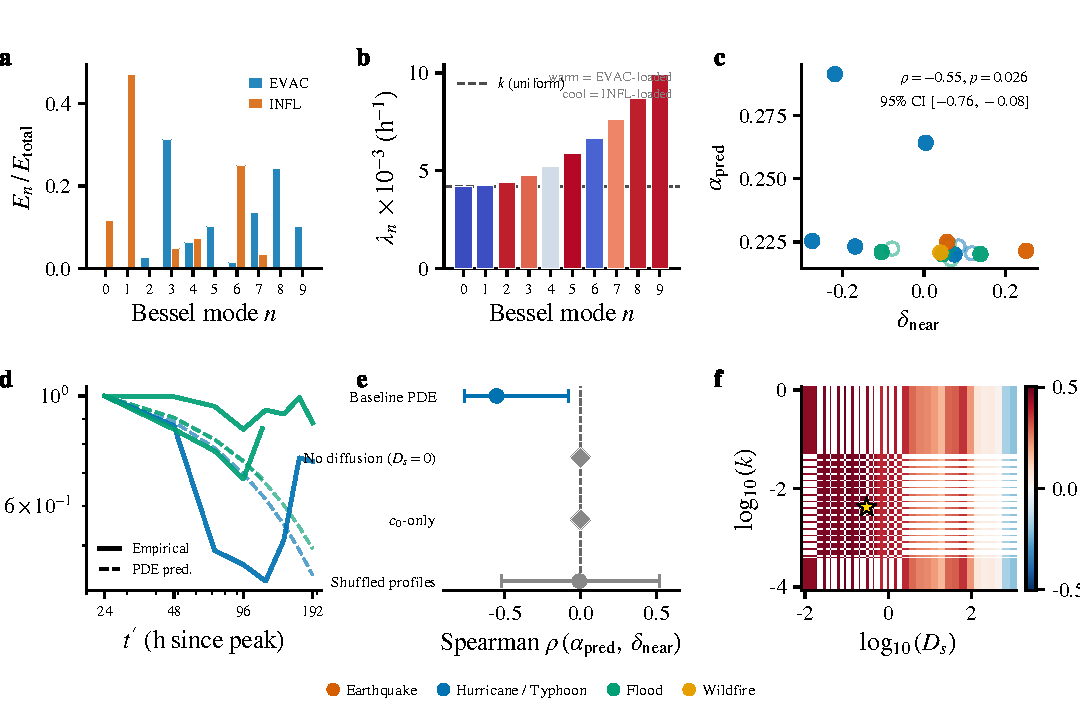
\includegraphics[width=\textwidth]{figures/fig3_pde_mechanism.pdf}
\caption{\textbf{A diffusion--relaxation model explains the shape--rate connection.}
\textbf{(a)}~Relative modal energy $E_n/E_{\mathrm{total}}$ for each Bessel
mode $n=0,\ldots,9$ for one EVAC representative (Beryl, Quintana Roo, blue) and one INFL
representative (2024 Spain flood, orange).  INFL profiles concentrate energy in the
low-frequency $n=1$ mode; EVAC profiles distribute energy broadly across
higher-order modes.
\textbf{(b)}~Mode decay rate $\lambda_n = k + D_s(\mu_n/R)^2$ (×$10^{-3}$ h$^{-1}$)
versus mode index.  The dashed line marks the uniform relaxation rate $k$;
higher modes decay faster owing to the diffusion term $D_s(\mu_n/R)^2$.
Bar colour encodes relative EVAC versus INFL energy loading (warm = EVAC-loaded).
\textbf{(c)}~Model-predicted decay rate $\apred$ versus $\dnear$.
$\rhosp = -0.55$ ($p = 0.026$); non-parametric bootstrap 95\%~CI
$[-0.76,\,-0.08]$ (98.4\% of realisations yield $\rhosp < 0$).
Open markers: events with $R^2 < 0.75$.
\textbf{(d)}~Predicted $\Dpred(t')$ (dashed) versus empirical
$\Demp(t')$ (solid) for three events (Beryl, Quintana Roo; 2024 Spain
flood; 2024 Central European flood), normalised at $t'=24$~h.
The model preserves event ranking but compresses variance by
approximately 15$\times$.
\textbf{(e)}~Counterfactual experiments: removing diffusion ($D_s=0$),
retaining only the uniform mode ($c_0$-only), or shuffling event--profile
pairings each eliminates $\rhosp$.  Filled circles: Spearman~$\rhosp$ with
bootstrap 95\%~CI; diamonds: deterministic scenarios.  Dashed line: $\rhosp=0$.
\textbf{(f)}~Parameter landscape: Spearman $\rho(\apred,\aemp)$ over the
$(\log k,\,\log D_s)$ grid.  Gold star marks the global optimum; the broad
plateau of high $\rho$ confirms robustness to parameter choice.}
\label{fig:pde}
\end{figure}

% ---- R4: D_peak ----
\FloatBarrier
\subsection*{Perturbation amplitude independently predicts recovery speed}

A second independent predictor---the perturbation amplitude~$\dpeak$,
the aggregated displacement at peak time---correlates positively with
recovery speed ($\rhosp = +0.60$, $p = 0.014$;
Fig.~\ref{fig:amplitude}a): larger disruptions recover faster.
The association is robust across all tested time-window definitions
($[24,72]$~h through $[24,144]$~h), Theil--Sen slope estimation, and
the model-free ratio~$D(72)/D(24)$ (Supplementary Table~S2).

Crucially, $\dpeak$ and $\dnear$ are statistically
independent ($\rhosp = -0.13$, $p = 0.63$): a large-amplitude event
is no more likely to be an evacuation-type than an influx-type event.
This orthogonality means the two predictors span genuinely complementary
dimensions of the initial disturbance.  In the two-dimensional
prediction space (Fig.~\ref{fig:amplitude}b), events separate into four
quadrants defined by the sample medians of $\dnear$ and $\dpeak$:
high-amplitude, evacuation-type events (upper left) cluster at the
highest recovery rates, whereas low-amplitude, influx-type events (lower
right) are slowest to recover.  The T\"{u}rkiye--Syria earthquake sits
in the low-amplitude, influx quadrant, consistent with its slow
recovery.  The quadrant structure shows that combining both peak-time
predictors substantially narrows the range of plausible recovery
trajectories.

Partial correlations confirm the independence of the two channels.
Controlling for~$\dnear$ leaves the amplitude--recovery link intact:
$\rhosp(\dpeak,\aemp \mid \dnear) = +0.63$, $p = 0.021$ (Supplementary
Table~S4).  Conversely, controlling for~$\dpeak$ preserves the
geometry--recovery link:
$\rhosp(\dnear,\aemp \mid \dpeak) = -0.57$, $p = 0.028$
(Supplementary Table~S4).  The PDE model produces predicted
rates~$\apred$ that show no statistically significant association
with~$\dpeak$ ($\rhosp = +0.39$, $p = 0.131$), confirming that the
amplitude effect arises from a mechanism outside spatial diffusion---the
model encodes geometry but is blind to magnitude.

\begin{figure}[t]
\centering
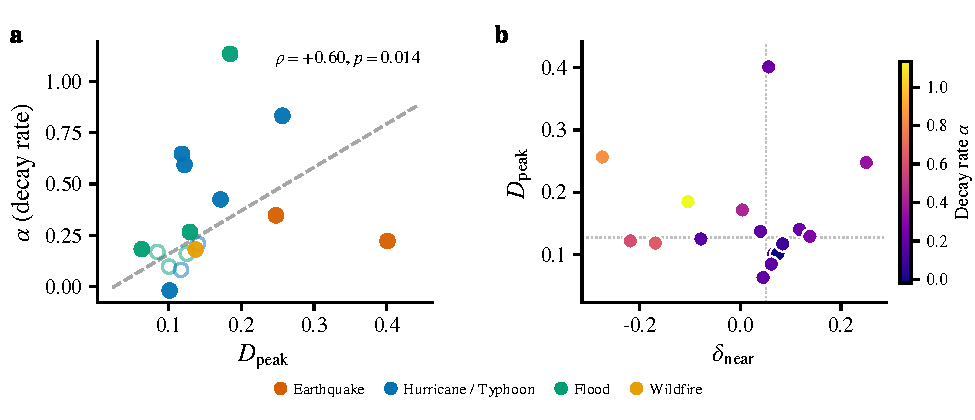
\includegraphics[width=\linewidth]{figures/fig4_amplitude_orthogonality.pdf}
\caption{\textbf{Perturbation amplitude independently predicts recovery speed.}
\textbf{(a)}~$\alpha$ versus $\dpeak$; open markers denote $R^2 < 0.75$.
\textbf{(b)}~Two-dimensional prediction framework: each point placed at
$(\dnear,\,\dpeak)$ and coloured by~$\alpha$.  Dotted lines mark sample
medians; high-$\alpha$ events (yellow/green) cluster in the upper-left quadrant
($\dnear < 0$, high $\dpeak$), consistent with independent
contributions.
\textbf{(c)}~Partial Spearman correlations of $\dnear$ with $\alpha$,
controlling sequentially for country-level HDI, GDP per capita PPP, and
INFORM risk sub-scores.  The geometry--recovery correlation
($\rhosp \in [-0.54,\,-0.52]$) is stable across all controls.
\textbf{(d)}~Partial Spearman correlations of $\dpeak$ with $\alpha$,
controlling for the same socioeconomic variables and additionally for
$\dnear$.  $\dpeak$ retains $\rhosp \in [+0.60,\,+0.63]$ throughout.
Panels~(a,b) correspond to the orthogonality analysis; panels~(c,d)
confirm socioeconomic invariance.}
\label{fig:amplitude}
\end{figure}


% ---- R5: Socioeconomic invariance ----
\FloatBarrier
\subsection*{Amplitude--recovery scaling is socioeconomic-invariant}

An alternative explanation is socioeconomic confounding: wealthier
societies might mount more effective evacuations, producing both larger
observed displacements and faster coordinated returns.  We test this
using country-level
HDI~(\citealt{UNDP2024}), GDP per capita PPP~(\citealt{WorldBank2024}),
and INFORM Risk sub-indices (Lack of Coping and
Vulnerability;~\citealt{INFORM2024}) for the 11~countries in our sample.
Because socioeconomic indicators are measured at the country level, events
from the same country share identical covariate values; results are
qualitatively identical when computed at the country level
($n = 11$; Supplementary \S6.5).

The data reject this hypothesis.  HDI ranges from 0.62~(Nepal) to
0.94~(USA), yet shows
essentially zero correlation with~$\dpeak$ ($\rhosp = 0.00$, $p =
1.00$) and negligible correlation with~$\aemp$ ($\rhosp = -0.11$,
$p = 0.68$).  GDP per capita PPP spans a 15-fold range from
\$5.7k~(Nepal) to \$85.8k~(USA), and likewise shows no association with
either variable.  The INFORM Lack of Coping sub-score---the indicator
most directly measuring institutional disaster-response
capacity---correlates with neither~$\dpeak$ nor~$\aemp$
(Table~\ref{tab:socioecon}).

Partial correlations (Fig.~\ref{fig:amplitude}c,d) show that the
amplitude--recovery link cannot be explained by latent national wealth
effects.  Controlling for HDI, GDP, or INFORM individually leaves the
$\dpeak$--$\aemp$ Spearman correlation essentially unchanged (from
$+0.60$ bivariate to a range of $+0.60$--$+0.62$ after conditioning;
Supplementary Table~S4).  The geometry--recovery link is equally
robust: $\rhosp(\dnear,\aemp)$ remains between $-0.52$ and $-0.54$
after conditioning on any single development indicator
(Fig.~\ref{fig:amplitude}c).
Controlling for~$\dnear$ and a development indicator simultaneously
yields $\rhosp \approx +0.63$
($p = 0.021$--$0.023$), slightly \emph{stronger} than the bivariate
estimate---a suppressor pattern indicating that development variation
contributes noise rather than signal to the amplitude--recovery
relationship.  The amplitude--recovery scaling is a feature of the
disturbance itself, not a reflection of differential national
development.

\begin{table}[t]
\centering
\caption{Bivariate Spearman correlations between socioeconomic
indicators and the two key analysis variables ($n = 16$ events from
$11$~countries).  No correlation reaches statistical significance
($p > 0.44$ for all).}
\label{tab:socioecon}
\small
\begin{tabular}{@{}lcccc@{}}
\toprule
Indicator & $\rhosp$ vs $\dpeak$ & $p$ & $\rhosp$ vs $\aemp$ & $p$ \\
\midrule
HDI                    & $+0.00$ & $1.00$ & $-0.11$ & $0.68$ \\
GDP per capita PPP     & $+0.01$ & $0.97$ & $-0.11$ & $0.67$ \\
INFORM Lack of Coping  & $-0.21$ & $0.44$ & $-0.04$ & $0.88$ \\
INFORM Vulnerability   & $+0.13$ & $0.64$ & $-0.11$ & $0.68$ \\
\bottomrule
\end{tabular}
\end{table}

% Partial correlation table moved to SI (Table S4)


% ============================================================
%  DISCUSSION
% ============================================================
\FloatBarrier
\section*{Discussion}

The results reveal shared structure in post-disaster population recovery
despite substantial hazard and country heterogeneity.  Two quantities---the spatial geometry of the
displacement profile ($\dnear$) and the perturbation
amplitude ($\dpeak$)---jointly predict recovery speed across earthquakes,
hurricanes, floods, and wildfires in 11~countries.  These predictors are
statistically independent ($\rhosp = -0.13$, $p = 0.63$), carry
distinct physical content, and have different levels of mechanistic
explanation.

\paragraph{Spatial diffusion as a recovery mechanism.}
The shape--rate connection is consistently explained by a minimal
diffusion--relaxation PDE whose counterfactual experiments
(Fig.~\ref{fig:pde}e) provide sharp mechanistic evidence: the signal
vanishes when diffusion is removed, when spatial structure is erased, or
when event--profile pairings are shuffled.  This connects post-disaster
population dynamics to the well-studied physics of relaxation in
diffusive systems~\citep{Crank1975}, where the rate of return to
equilibrium depends on the initial perturbation's spatial frequency
content.  The result is compatible with---but distinct from---the
hyperbolic spatial decay laws identified by \citet{Li2022} for
mobility deviations during crises: where \citet{Li2022} characterise
the spatial envelope of crisis-induced deviations at a fixed time, our
PDE framework links the \emph{temporal} rate of decay to the
\emph{spatial} structure of the initial disturbance.  Together the two
frameworks suggest a coherent picture in which spatial profile shape and
temporal decay are coupled through diffusive relaxation.  The empirical
power-law decay we document---slower than the pure exponential predicted
by a single-mode model---is consistent with the broader finding that
recovery dynamics in complex systems carry memory and non-Markovian
features that extend relaxation times~\citep{Lin2020}.

\paragraph{Why do larger perturbations recover faster?}
The amplitude--recovery scaling is robust but less constrained
mechanistically.  Similar amplitude-dependent recovery appears in other
perturbed systems with active restoring forces.  In financial markets,
larger initial volatility shocks after Covid-19 were associated with
shorter recovery times through stronger mean-reversion
forces~\citep{Zeng2024}; and price adjustment across many products
shows that larger shocks propagate faster because they trigger stronger
state-dependent responses~\citep{Cavallo2024}.  In infrastructure
systems, wider-area power outages can exhibit faster probabilistic
restoration when large events trigger mutual-aid protocols that scale
nonlinearly with affected area~\citep{Willems2024,Afsharinejad2021}.
Even in post-fire ecosystems, higher burn severity accelerates
vegetation recovery through accelerated nutrient cycling~\citep{Qiu2023}.
These cross-domain parallels point to a general principle: large
perturbations activate qualitatively stronger restoration regimes.
For disaster displacement, plausible channels include super-linear
scaling of emergency response with event severity~\citep{Eisensee2007,Stromberg2007}
and stronger behavioural reversion toward habitual mobility states
after severe disruption~\citep{Gonzalez2008}.  What our data
establish directly is that this scaling is \emph{not} mediated by
national socioeconomic conditions.

\paragraph{Recovery as incomplete return.}
Post-disaster recovery does not invariably mean return to the
pre-event baseline.  The residual
displacement~$D_\infty$---the normalised mean of $D(t)$ over the
post-peak tail---is non-zero for most events, indicating that some
fraction of displaced populations do not return within the two-week
observation window.  The strong anticorrelation between~$\aemp$
and~$D_\infty$ ($\rhosp = -0.703$, $p = 0.002$; Supplementary
\S6.4; Fig.~\ref{fig:relaxation}d) means that fast-recovering events also converge to lower
residuals: the same mechanisms that accelerate return also deliver more
complete return.  For slow-recovering events, the elevated residual
may signal a new stable population configuration---a temporary or
permanent displaced equilibrium---rather than a recovery trajectory
that simply has not yet completed.  Distinguishing between these
interpretations requires observation windows substantially longer than
two weeks and integration with data on household resettlement, housing
reconstruction, and long-term migration.

\paragraph{From two predictors to a prediction framework.}
The shape--rate and amplitude--rate associations are not merely two
separate findings; their statistical independence means they span
complementary axes of a prediction space.  At the moment of peak
displacement---often within the first few days of the event---both
$\dnear$ and $\dpeak$ are observable from near-real-time FBDM tiles,
and together they partition events from fastest recovery (large
amplitude, evacuation pattern) to slowest (small amplitude, influx
pattern).  This reframes early post-disaster assessment from
retrospective narrative to prospective quantification: the recovery
trajectory is substantially encoded in the initial condition, before
the full effects of institutional response, aid delivery, or
reconstruction policy have accumulated.

\paragraph{Limitations and outlook.}
Our sample of 16~events, while spanning diverse hazard types and
development contexts, remains modest and is subject to FBDM activation
decisions.  Facebook Disaster Maps measures movements of Facebook users,
who skew toward urban, younger, and more connected segments of the
population; such demographic skew in mobile-data platforms is known to
bias modeled mobility dynamics~\citep{Chin2025,Gallotti2024}, and
coverage varies substantially by country and by local platform
adoption~\citep{Huang2025}.  Observation windows of roughly two weeks
capture acute recovery dynamics but not long-term reconstruction or
subsequent displacement cycles.  The socioeconomic analysis operates at
national scale (effective $n = 11$~countries), masking sub-national
heterogeneity that may be substantial---a community-level analysis
would require matched community-level development indicators.  The
radial-annulus framework is most natural for point-source hazards such
as earthquakes; for spatially diffuse events (floods, wildfires), the
choice of epicenter introduces additional geometric uncertainty.
Inference is also aggregate (tile $\rightarrow$ annulus $\rightarrow$
event): individual-level mobility decisions cannot be identified from
these event-level statistics alone.  The
shape--rate hypothesis is pre-specified from the PDE model's physical
prediction and withstands multiple independent robustness checks; the
amplitude--recovery scaling is an empirical discovery whose mechanistic
basis---whether super-linear restoring forces, intrinsic mean-reversion,
or a combination---remains a target for future investigation with larger
samples, longer observation windows, and finer-grained socioeconomic
and infrastructure data.


\FloatBarrier
% ============================================================
%  MATERIALS AND METHODS
% ============================================================
\section*{Materials and Methods}

\paragraph{Data.}
We use Facebook Disaster Maps~\citep{Maas2019}, which provide
tile-level (${\sim}2.4$~km) population density estimates at 8-hour
resolution for disaster-activated regions.  For each event, tiles within
$R = 200$~km of the estimated event center are binned into 10-km radial
annuli.  Event centers are determined as follows: for earthquakes, the
catalogued epicenter is used; for hurricanes and typhoons, the track
anchor at landfall or closest approach; for floods and wildfires, the
population-weighted centroid of tiles with the largest absolute density
change.  The population ratio
$\phi_{r,t} = n_{\mathrm{crisis}} / n_{\mathrm{baseline}}$
is averaged within each annulus; annuli with fewer than 3~populated tiles
are excluded.  The baseline count~$n_{\mathrm{baseline}}$ is the
platform-provided pre-event mean, computed by FBDM over the 90~days
preceding map activation, stratified by day of week and 8-hour time
window.  The aggregated displacement metric is defined as the mean
absolute deviation across retained radial bins:
\begin{equation}
  D(t) = \bigl\langle\,|\phi_{r,t} - 1|\,\bigr\rangle_r .
  \label{eq:Dt}
\end{equation}

\paragraph{Event selection.}
Approximately 35~disaster events with FBDM coverage (2020--2025) were
screened for analytical suitability.  Events were retained if they had
(i) sufficient tile coverage within the 200-km analysis disk ($\geq 3$
populated tiles per annulus at peak), (ii) a clearly identifiable single
peak in~$D(t)$, and (iii) a monotone-decay segment of at least three
post-peak time steps ($n_{\mathrm{mono}} \geq 3$).  Events representing
the same physical disaster through multiple separate FBDM deployments
(e.g.\ Rio Grande do Sul flooding, Hurricane Melissa aftermath) were
consolidated to a single entry to avoid pseudo-replication.  The final sample comprises 16~events spanning
four hazard types (earthquake, hurricane/typhoon, flood, wildfire) in
11~countries (Supplementary Table~S1).

\paragraph{Peak displacement $\dpeak$ and residual displacement $D_\infty$.}
$\dpeak = \max_t D(t)$ is the peak of the aggregated displacement curve.
The residual displacement $D_\infty$ is defined as the mean of the
normalised curve $D(t')/\dpeak$ over the post-peak tail
($t' > 0.5\,t_{\mathrm{obs}}$), where $t_{\mathrm{obs}}$ is the total
post-peak observation length; $D_\infty = 0$ would indicate complete
return to baseline.

\paragraph{Decay rate $\alpha$.}
After $D(t)$ reaches its peak, the normalized curve
$\Dnorm(t') = D(t')/\dpeak$ is fitted to the power-law model
\begin{equation}
  \Dnorm(t') = (t'/t_0)^{-\aemp},
  \label{eq:powerlaw}
\end{equation}
by ordinary least squares on $\log\Dnorm$ versus $\log t'$.  The fit
is performed over the initial monotone-decay segment, starting at
$t' = 24$~h and truncated at the first structural rebound---defined
operationally as the first time step at which
$D_{\mathrm{norm},i+1} > 1.05\,D_{\mathrm{norm},i}$ (i.e.\ a 5\%
bounce tolerance; details in SI~\S1).  We choose the power-law form
over alternatives (exponential, stretched-exponential) on the basis of
Bayesian Information Criterion comparisons across all 16~events: the
power law achieves lower BIC in 13 of 16~events (Supplementary
Table~S2a), consistent with the scale-free decay documented in
crisis-mobility studies~\citep{Li2022} and in contrast to exponential
decay, which would predict the same characteristic time irrespective
of perturbation scale.  Robustness is confirmed across four fixed time
windows ($[24,72]$~h through $[24,144]$~h), Theil--Sen robust
regression~\citep{Sen1968}, and a model-free ratio $D(72)/D(24)$
used as an alternative non-parametric measure of decay speed
in the same correlation analyses (Supplementary Table~S2b).
Events with $R^2 < 0.75$ (four events; $\dagger$ in Table~S1) are
retained in all analyses and shown with open markers; the primary
correlations are qualitatively unchanged when they are excluded
(Supplementary \S6.2).

\paragraph{Near-field displacement direction $\dnear$.}
$\dnear$ is the mean of
$\delta(r) = \phi(r, t) - 1$ over $r < 50$~km, averaged across all
time windows in which $D(t) \geq 0.5\,\dpeak$ (i.e.\ the peak plateau),
requiring at least two populated near-field annuli per time step.

\paragraph{PDE model.}
Equation~\eqref{eq:pde} is solved analytically under Neumann
(zero-flux) boundary conditions on a disk of radius $R = 200$~km.  The
solution decomposes into Bessel $J_0$ modes:
\begin{equation}
  \delta(r,t) = \sum_{n=0}^{N-1} c_n\,J_0\!\left(\frac{\mu_n r}{R}\right)
    e^{-\lambda_n t},
  \label{eq:bessel}
\end{equation}
where $\mu_n$ are the zeros of $J_0'$ (with $\mu_0 = 0$ for the
spatially uniform fundamental mode), each mode decays at rate
$\lambda_n = k + \Ds(\mu_n/R)^2$, and $N = 10$ modes are retained
(convergence checked up to $N = 20$).  Initial coefficients~$\{c_n\}$
are determined from each event's observed radial profile at
$t_{\mathrm{peak}}$ via $r$-weighted least-squares projection.

The predicted energy decay is defined as
$E(t) = \langle\delta^2\rangle_r = \sum_{n} c_n^2\,e^{-2\lambda_n t}$,
the $L_2$ (mean-square) norm of the displacement field.  We fit $E(t)$
rather than $D(t)$ on log--log axes over $[1,120]$~h to obtain the
predicted rate~$\apred$, because $E(t)$ has an exact analytical form
under the Bessel decomposition (Parseval's relation), whereas the
$L_1$ metric $D(t) = \langle|\delta|\rangle_r$ does not.  The
systematic variance compression by~${\sim}15{\times}$ between~$\apred$
and~$\aemp$ is expected: the $L_2$ metric amplifies high-frequency
modes relative to $L_1$, inflating the predicted range of decay rates
beyond what is empirically observed in the $L_1$ metric.

The two global parameters, $k$ and $\Ds$, are found by grid search
over a $30 \times 30$ logarithmic grid spanning
$k \in [10^{-4},\,10^{0}]$~h$^{-1}$ and
$\Ds \in [10^{-2},\,10]$~km$^2$\,h$^{-1}$.  The criterion minimised
is a joint rank score combining three components weighted equally:
(i) the negative Spearman correlation between~$\apred$ and~$\aemp$
across all 16~events, (ii) the negative Pearson correlation, and
(iii) the mean absolute error between~$\apred$ and~$\aemp$.  Weighting
Spearman alongside Pearson ensures robustness to outliers; including
MAE prevents the criterion from ignoring scale.  The selected
parameters, $k = 0.0042$~h$^{-1}$ and $\Ds = 0.30$~km$^2$\,h$^{-1}$,
reside in a broad plateau of the criterion landscape (Supplementary
\S3), indicating that the result is not sensitive to the exact
parameter values.

\paragraph{Counterfactual experiments.}
Three counterfactual scenarios test the necessity of the model's
ingredients: (i)~\emph{no diffusion} ($\Ds = 0$): all modes decay at
the uniform rate~$k$, removing mode-selective damping;
(ii)~\emph{uniform mode only} ($c_0$-only): the observed spatial
structure is replaced by a flat perturbation, retaining diffusion but
erasing spatial content; (iii)~\emph{shuffle}: event--profile pairings
are randomised ($n = 500$ permutations), breaking the link between each
event's own geometry and its recovery history.

\paragraph{Temporal prediction $\Dpred(t)$.}
For each event, the fitted Bessel expansion~\eqref{eq:bessel} is
propagated forward from $t_{\mathrm{peak}}$ and aggregated to the
predicted displacement trajectory
$\Dpred(t') = \langle\,|\delta(r,t')|\,\rangle_r$, evaluated
numerically over the same radial grid used for the initial projection.
Both $\Dpred(t')$ and $\Demp(t')$ are normalised at $t' = 24$~h for
direct comparison.

\paragraph{Socioeconomic data.}
Country-level indicators---HDI~\citep{UNDP2024}, GDP per capita PPP
\citep{WorldBank2024}, and INFORM sub-scores~\citep{INFORM2024}---are
matched to the 11~countries hosting the 16~events.  Partial Spearman
correlations control for one or more indicators simultaneously (SI~\S4).

\paragraph{Statistical tests.}
All correlations are Spearman rank unless otherwise noted.  Significance
thresholds are two-sided at $p < 0.05$.  Mann--Whitney $U$ tests compare
$\aemp$ distributions between EVAC and INFL events
(Fig.~\ref{fig:shape}d).  Robustness checks include
leave-one-out jackknife (95\% CI), $r_{\mathrm{near}}$
sweeps from 10 to 200~km, $R_{\max}$ sweeps from 50 to 400~km, and
a non-parametric bootstrap ($n = 500$ realisations) over
initial-profile perturbations drawn from the tile-level noise
distribution.  Partial Spearman correlations are computed via
rank-transform-and-regress~\citep{Conover1999}: variables are replaced
by their ranks, ordinary least-squares residuals are obtained, and
Spearman correlation is computed on the residualised ranks.

Because different events have different post-peak observation lengths,
$D_\infty$ is computed over the second half of each event's available
post-peak window.  The resulting values are comparable across events
because $\Dnorm(t')$ is normalised by $\dpeak$ before averaging.

\paragraph{Software.}
All analyses were performed in Python~3.11 using NumPy~1.26,
SciPy~1.12, pandas~2.2, and Matplotlib~3.9.  Bessel function zeros
and special functions are from \texttt{scipy.special}.


% ============================================================
%  DATA AND CODE AVAILABILITY
% ============================================================
\section*{Data availability}
Facebook Disaster Maps data were obtained through Meta's Data for Good
programme.  Access requires an institutional agreement with Meta;
requests can be submitted at
\url{https://dataforgood.facebook.com/}.  Processed, event-level
summary statistics (radial profiles, decay rates, Bessel coefficients,
socioeconomic indicators) sufficient to reproduce all figures and
tables are available at [Zenodo DOI to be inserted upon acceptance].

\section*{Code availability}
Analysis code (Python) for data processing, PDE modelling, figure
generation, and statistical tests is available at
[GitHub/Zenodo link to be inserted upon acceptance].

% ============================================================
%  ACKNOWLEDGMENTS
% ============================================================
\section*{Acknowledgments}
We thank Meta for making Facebook Disaster Maps data available for
research.  [Funding information to be added.]

% ============================================================
%  REFERENCES
% ============================================================
\small
\bibliographystyle{unsrtnat}
\bibliography{references}

\end{document}
